\section{Methods}
\label{sec:methods}

\paragraph{Research Methodology}
The research will be conducted through a literature review of scientific articles, conference papers and thesis if available.
The main sources of information will be the IEEE Xplore, ScienceDirect, and Google Scholar databases.
The search will be conducted using the following keywords: "Chip-Scale Atomic Clock", "Atomic Clock", "MEMS", "CSAC", "Vapor Cell", "Rubidium", "Cesium", "Microwave Cavity", "Laser Cooling", "Photon Detector", "Quartz Crystal Oscillator", "Electron Spin", "Electron Excitation", "Optical Lattice Clock", "Quantum Technologies".

During the research, we will try to annotate the most relevant papers and articles, that will be then used to write the final report.

\paragraph{Outline}
We leave here a general outline that will be used as a guide for the development of the project.

\begin{enumerate}
    \item Introduction: Discuss the need for precise timekeeping and the exigence of chip-scale atomic clocks.
    \item \textbf{Engineering of Chip-Scale Atomic Clocks}: Discuss the principles of operation. Note: It would be interesting to use simulation tools such as \texttt{COMSOL Multiphysics} to visualize the operating principles of these devices, but not knowing the software and its capabilities, I am not sure if it is applicable here.
          \begin{itemize}
              \item Vapour cell
              \item Magnetic selector (electron spin)
              \item Microwave cavity (electron excitation at hyperfine transition)
              \item Laser system (laser cooling and trapping of atoms)
              \item Photon detector
              \item Closed loop over quartz crystal oscillator
          \end{itemize}
          \begin{figure}[H]
              \centering
              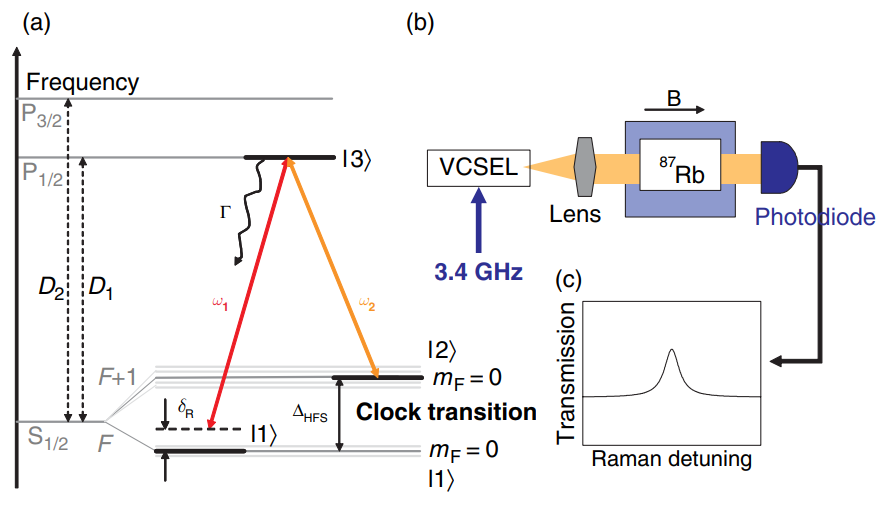
\includegraphics[width=.6\textwidth]{img/atomic_clock_logic}
              \caption{Schematic of the simplified atomic energy level configuration \cite{KNAPPE2008571}}
          \end{figure}

    \item \textbf{Technology Comparison}: Introduce the different types of chip-scale atomic clocks. Compare and contrast the different chip-scale atomic clock technologies in terms of size, power consumption, accuracy, and suitability for various applications.
          \begin{itemize}
              \item Cesium based
              \item Rubidium based
          \end{itemize}
          % \item Fabrication and Manufacturing: Explore the components of chip-scale atomic clocks such as atomic vapor cells, laser systems, and control electronics. Understand the microfabrication techniques used in their manufacturing.
    \item Applications: Consider the diverse applications of chip-scale atomic clocks (aerospace and defense to telecommunications and scientific research)
    \item Challenges and Future Directions: Identify current challenges such as size reduction and power efficiency, and consider future trends like adoption of optical lattice clocks and integration with quantum technologies.
    \item Conclusion: Summarize the key findings of the research and discuss the implications for future advancements and applications of chip-scale atomic clocks.
\end{enumerate}

% In case of time availability, we will also cover the Fabrication and Manufacturing of these devices, understanding the microfabrication techniques used in their manufacturing.

\paragraph{Time schedule}
In general, given a time constraint of 4/5 weeks, the project will be divided as follows (tentative)

\begin{itemize}
    \item Week 1: Introduction + Engineering of Chip-Scale Atomic Clocks
    \item Week 2: Engineering of Chip-Scale Atomic Clocks (possible simulation and results analysis)
    \item Week 3: Technology Comparison + Applications
    \item Week 4: Challenges and Future Directions + Conclusion
    \item Week 5: Final report writing
\end{itemize}
